\documentclass[12pt]{article}
\usepackage{geometry}                % See geometry.pdf to learn the layout options. There are lots.
\geometry{letterpaper}                   % ... or a4paper or a5paper or ... 
%\geometry{landscape}                % Activate for for rotated page geometry
\usepackage[parfill]{parskip}    % Activate to begin paragraphs with an empty line rather than an indent
\usepackage{daves,fancyhdr,natbib,graphicx,dcolumn,amsmath,lastpage,url}
\usepackage{amsmath,amssymb,epstopdf,longtable}
\usepackage[final]{pdfpages}
\DeclareGraphicsRule{.tif}{png}{.png}{`convert #1 `dirname #1`/`basename #1 .tif`.png}
\pagestyle{fancy}
\lhead{CE 3372 -- Water Systems Design}
\rhead{SPRING 2025}
\lfoot{PR1}
\cfoot{}
\rfoot{Page \thepage\ of \pageref{LastPage}}
\renewcommand\headrulewidth{0pt}



\begin{document}
\begin{center}
{\textbf{{ CE 3372 Engineering Hydrology} \\ {Project PR1}}}
\end{center}

\section*{Project Overview:}
The City of Pecos, Texas, has identified a critical need to develop an alternate water supply in anticipation of the current wellfield reaching the end of its service life within the next 5-10 years. To ensure the city's long-term water security, an alternate wellfield has been identified, and property rights for its development have been secured. This wellfield is located approximately 30 miles south of the city center.

Your task is to design the components necessary to transport water from this alternate wellfield to Pecos and ensure adequate storage for future demand. This design includes:

\begin{enumerate}
\item Wellfield Collector Network: Design the network of wells and collection lines that will efficiently gather water from the wellfield and deliver it to a central collection point.
\item Transmission Pipeline: Design the transmission pipeline system that will carry water from the wellfield to the city’s water treatment and distribution facilities. Consider hydraulic design principles to size the pipeline appropriately based on flow rates and friction losses over the 30-mile distance.
\item Storage Facilities: Design intermediate storage facilities as necessary, as well as terminal storage to ensure there is sufficient water available for city consumption during peak demand periods or in case of pipeline interruptions. Storage should accommodate both daily use and emergency reserves.
\end{enumerate}

Assumptions and Constraints:

    The city currently uses approximately 2.7 million gallons per day (MGD), with a peak usage of 3.9 MGD and projected growth should be accounted for over a 20-year horizon.
    The alternate wellfield is estimated to produce up to 3.024 MGD, with fluctuations due to seasonal variations.
    Transmission pipeline materials and layout should be designed considering local terrain and minimizing environmental impacts.
    Intermediate storage facilities may be required based on pipeline hydraulic design and system pressures.
    Air entry and pressure relief facilities may be required based on pipeline hydraulic design and system pressures.

Deliverables:

\begin{itemize}
\item Design the wellfield pipe network to the collector point. The well locations are already established from a preliminary study conducted during the water rights acquistion process.
\item Size the transmission pipeline and provide justification for your selection (e.g., diameter, material).  The approximate alignment is attached, the design should include appropriate burial depths for the pipeline at locations along the alignment, as well as actual pipeline elevations.  A topographic profile along the alignment is required as an aid to locating pressure relief facilities along the 25+ mile pipeline.
\item Determine the volume of intermediate and terminal storage facilities required and provide recommendations on their placement.
\item Demonstrate using a hydraulic model that the system can deliver the required raw water to replace the existing supply, under variable demand conditions.  Identify using the model locations of low pressure, and high pressure. Produce plots of the energy grade line under various demsnd conditions.  Identify locations where pressure relief valves, air relief valves, and flow-control valves are required.
\item Determine and demonstrate an operating schedule to maintain positive pressure in the pipeline under varying flow conditions, and prevent storage tank overflows and complete tank drainage.
\item Determine using water-hammer analysis the anticipated pressure changes during sudden shutdown of the transmission pipeline.
\end{itemize}

Submission Requirements:
\begin{itemize}
\item A detailed design report with calculations, maps, and diagrams to support your wellfield, pipeline, and storage facility designs. The report must explain the rationale behind your design decisions, including considerations of cost, energy use, and reliability.
\item A final presentation summarizing your design choices, challenges, and proposed solutions.
\end{itemize}

Additional Information:
\begin{itemize}
\item West Pecos Water System (Proposed Alignment) (page 3)
\item West Pecos Wellfield (Well Locations and Collection Network) (page 4)
\item West Pecos Wellfield Pump Performance Curve (One per well) (page 5)
\item West Pecos Wellfield Pump Performance Table (Tabular version of pump curve) (page 6)
\item West Pecos Water System (KMZ file) \url{http://54.243.252.9/ce-3372-webroot/2-Exercises/PR1_PecosWater/WEST PECOS WATER SYSTEM.kmz}\footnote{A KMZ file is a compressed archive of multiple files, including a Keyhole Markup Language (KML) file and supporting files, that can be used to store and share geographic data}

\end{itemize}


\clearpage

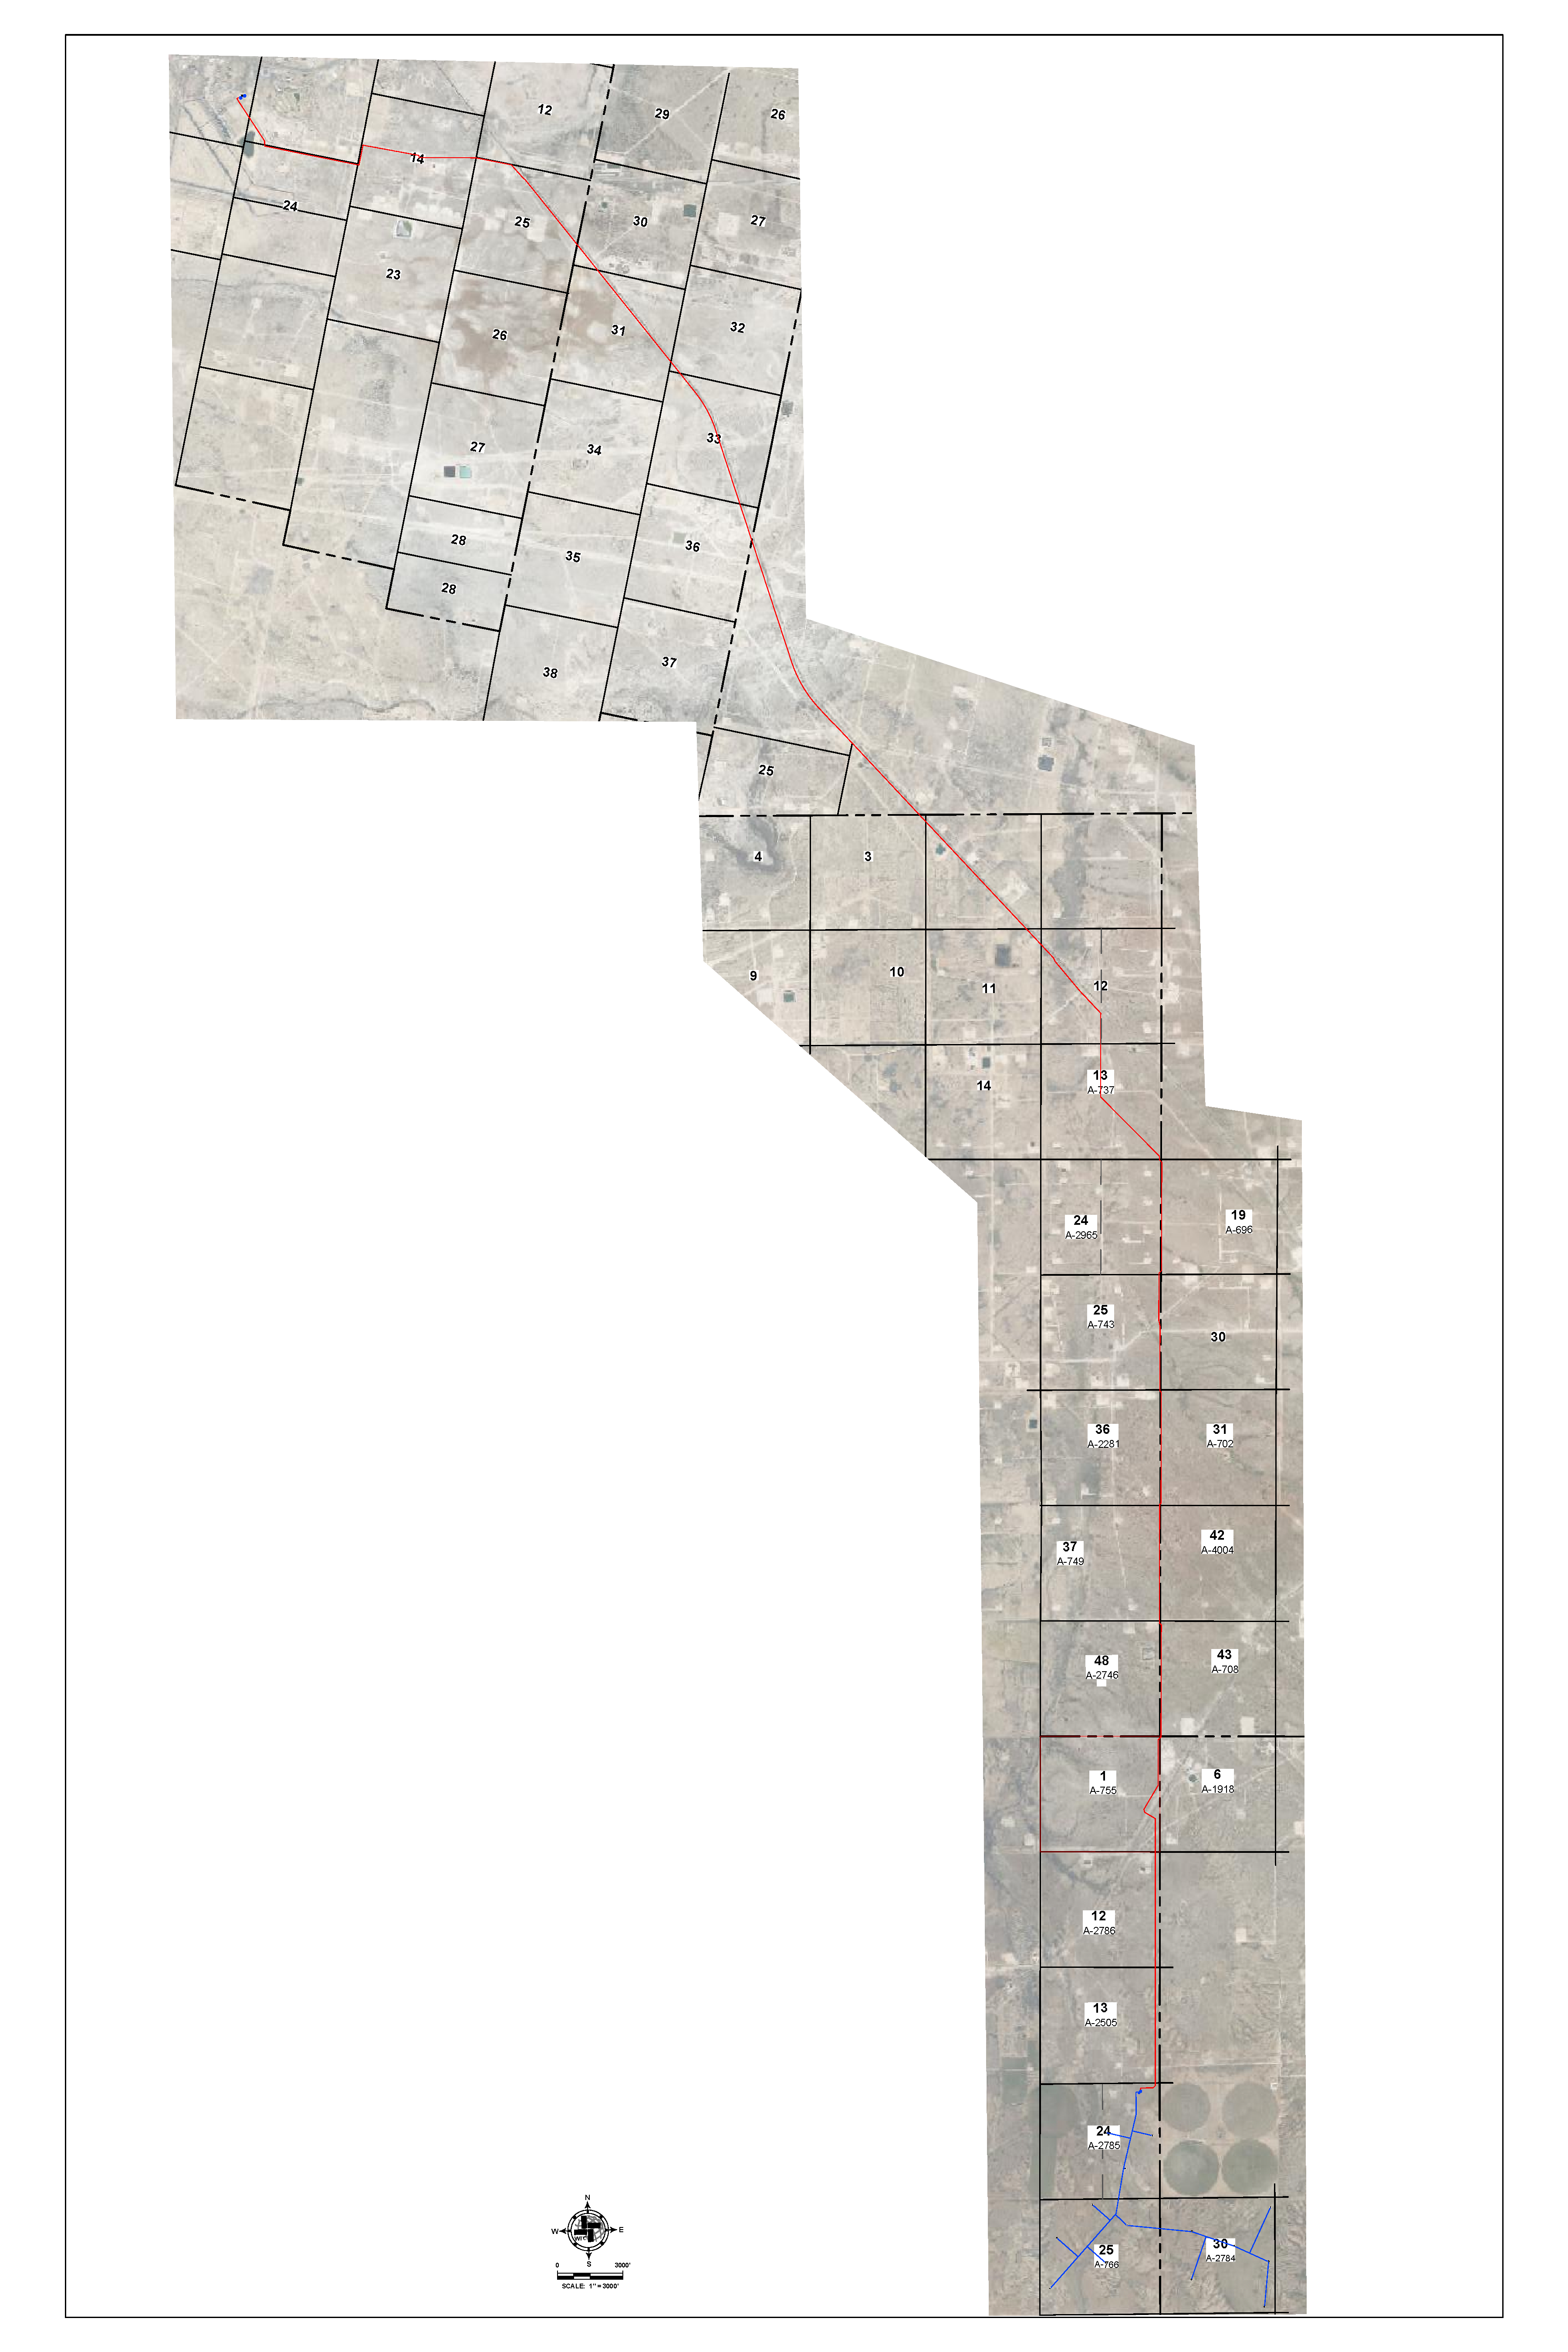
\includegraphics[
  page=1,
  width=\textwidth,
  height=\textheight,
  keepaspectratio,
  trim=0 0 0 20pt,
]{./WEST_PECOS_WATER_SYSTEM.pdf}

\clearpage

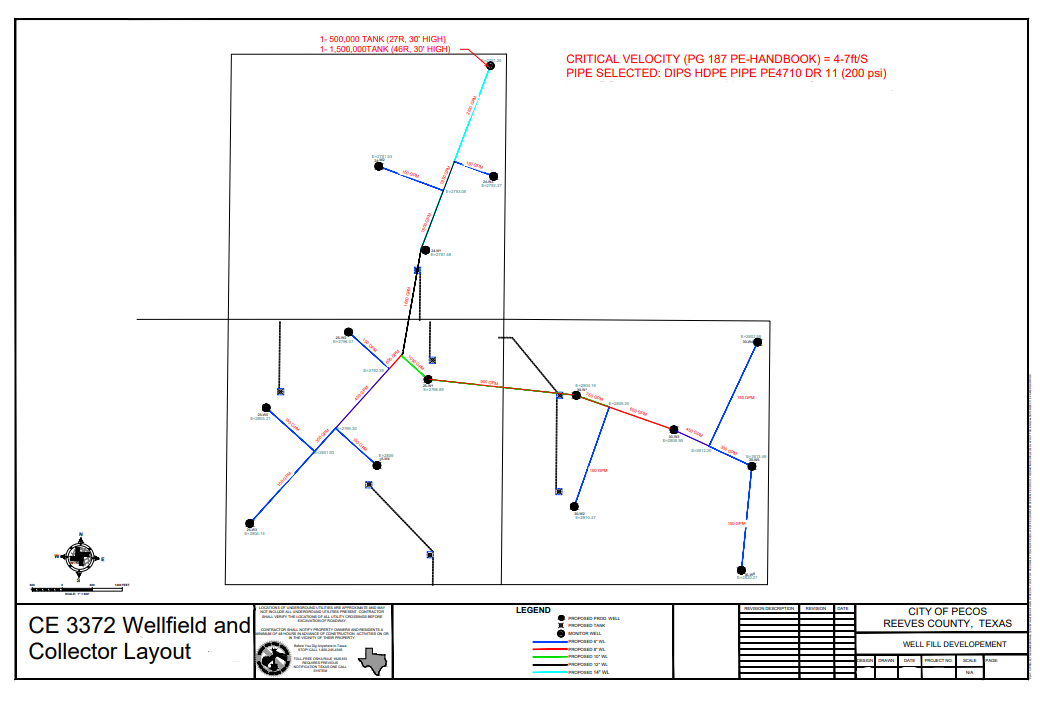
\includegraphics[
  page=1,
  width=\textwidth,
  height=\textheight,
  keepaspectratio,
  trim=0 0 0 20pt,
]{./Wellfield.png}

\clearpage

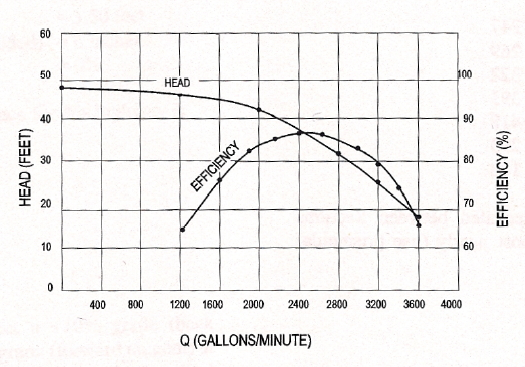
\includegraphics[
  page=1,
  width=\textwidth,
  height=\textheight,
  keepaspectratio,
  trim=0 0 0 20pt,
]{./PumpCurve.png}

\clearpage

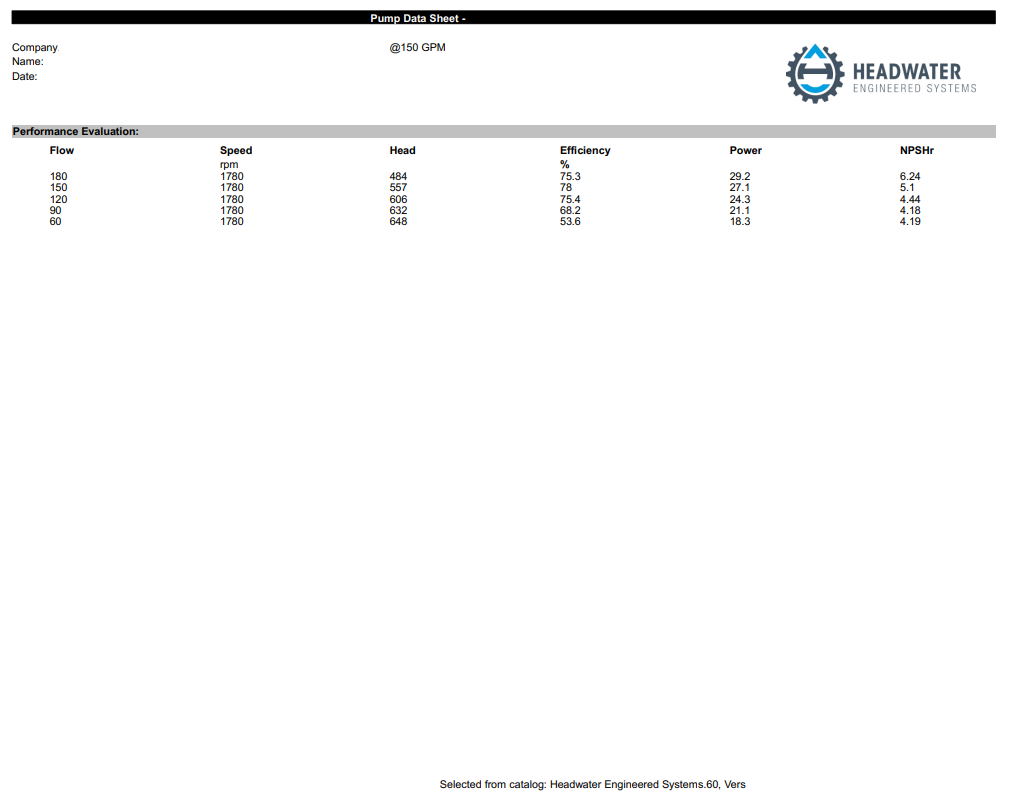
\includegraphics[
  page=1,
  width=\textwidth,
  height=\textheight,
  keepaspectratio,
  trim=0 0 0 20pt,
]{./PumpTabular.png}

%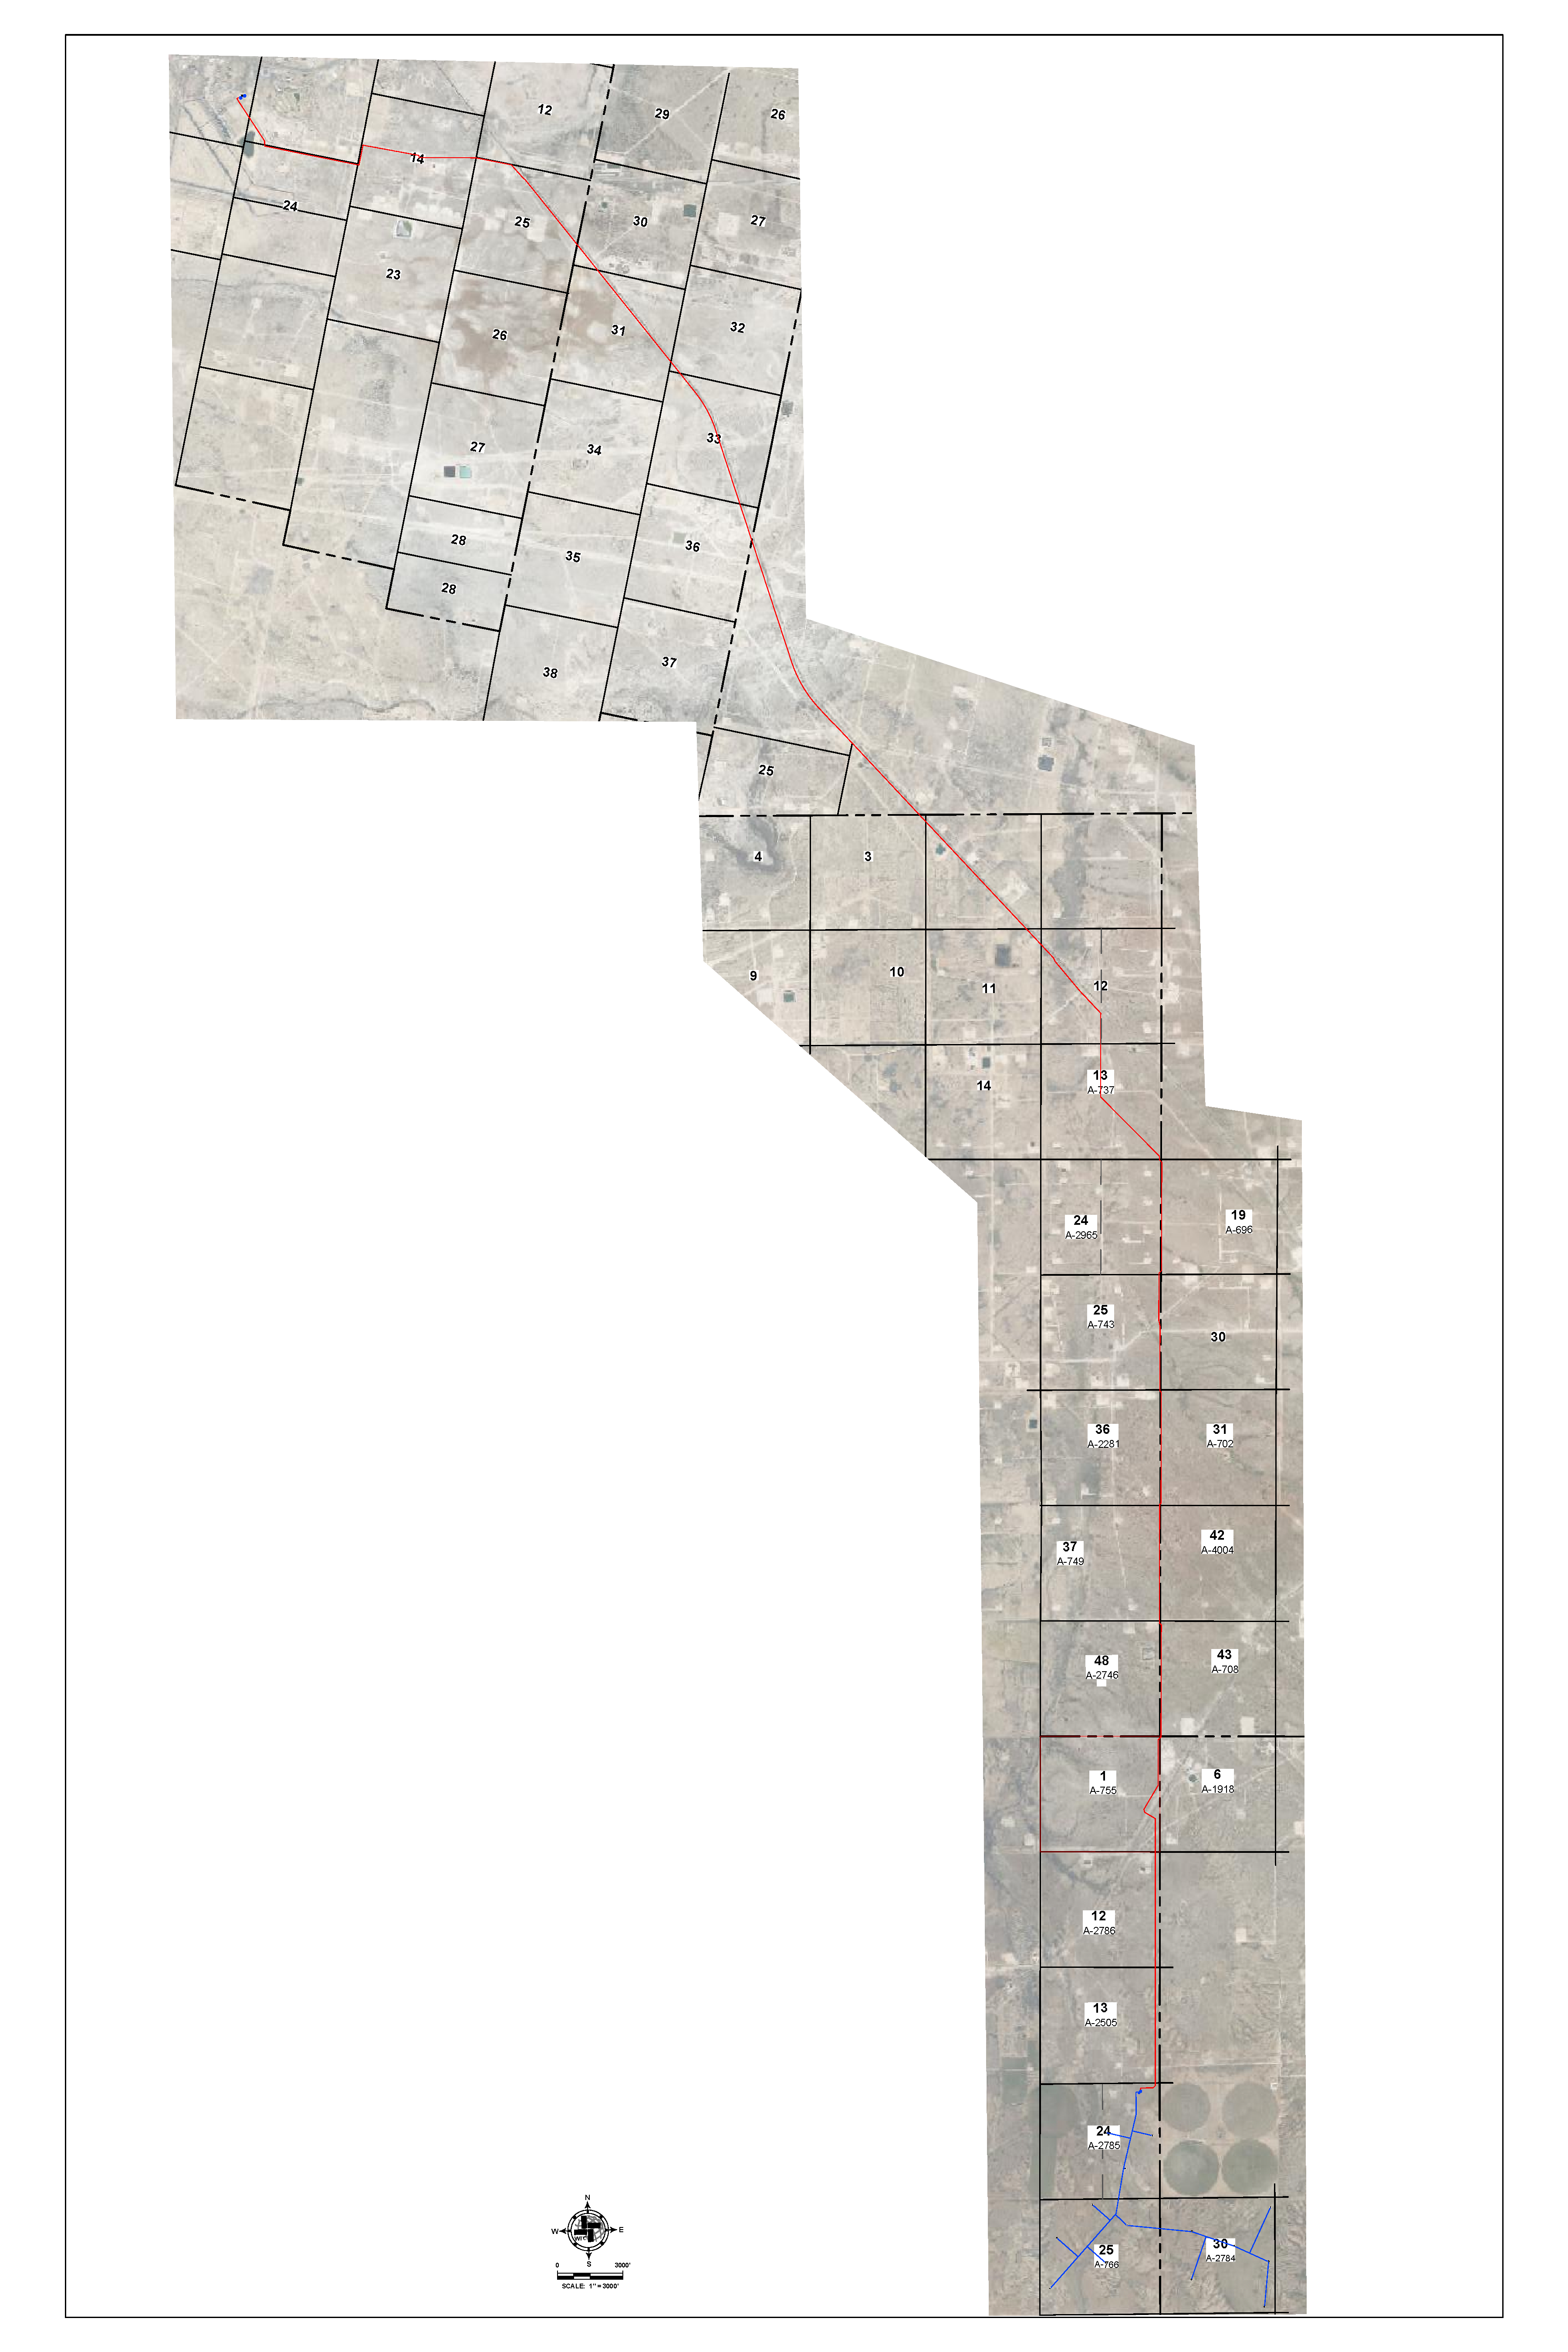
\includepdf[pages=-]{./WEST_PECOS_WATER_SYSTEM.pdf}
\end{document}  